%ullright document template
%default a4 one-sided article page setup
\documentclass[article, a4paper, oneside, 11pt]{memoir}

%the following three commands are necessary when using pdflatex
%(set input/output encoding)
\usepackage[utf8]{inputenc}
\usepackage[T1]{fontenc}
\usepackage{helvet}
%use sans serife font for body 
\renewcommand*\familydefault{\sfdefault}

%but with more tech-doc like margins
\setlrmarginsandblock{2.8cm}{2.8cm}{*}
\checkandfixthelayout

%for the german language
\usepackage[ngerman]{babel}

%including pictures
\usepackage{graphicx}
\graphicspath{{./figures/}}

%wrapping text around figures
\usepackage{wrapfig}

%url handling
\usepackage{url}

%elaborate references
\usepackage[ngerman]{varioref}

%we do not use xelatex anymore
%allows convenient font/color specification
%\usepackage{xcolor}
%\usepackage{fontspec}
%'classic' tex mappings, e.g. -- => en-dash
%\defaultfontfeatures{Mapping=tex-text}
%\setromanfont{Gentium Basic}
%\definecolor{DocBlue}{rgb}{0.1, 0.42, 0.59}
%\setsansfont[Color = DocBlue]{Ubuntu}

%enables pdf linking and attributes
\usepackage{hyperref}
\hypersetup{
    colorlinks=true,%
    citecolor=black,%
    filecolor=black,%
    linkcolor=black,%
    urlcolor=black
    pdfauthor={ull.at},%
    pdftitle={ullCms Handbuch},%
    pdfsubject={ullright - ullCms}
}

\chapterstyle{veelo}
\headstyles{komalike}
\pagestyle{empty}

%header and footer images on every page
\usepackage{wallpaper}
\ULCornerWallPaper{1.0}{header}
\LLCornerWallPaper{1.0}{footer}

%Precise figure placement
% \usepackage{float}

%padding for fbox borders
%\setlength\fboxsep{0pt}

%color headlines
\usepackage{color}
\usepackage{titlesec}

\definecolor{ullblue}{rgb}{0.1, 0.42, 0.59}

\titleformat{\chapter}[display]
{\color{ullblue}\normalfont\huge\bfseries}{\chaptertitlename\
\thechapter}{20pt}{\Huge}

\titleformat{\section}
{\color{ullblue}\normalfont\Large\bfseries}{\thesection}{1em}{}

% Do not indent paragraphes but add newlines
\usepackage{parskip}
\setlength{\parindent}{0cm}
\setlength{\parskip}{2mm}


%memoir recommendation
\clubpenalty=10000
\widowpenalty=10000
\raggedbottom


\begin{document}

\vspace*{3cm}
%move picture left/right
\begin{figure}[htp]
\centering

\includegraphics[width=0.5\textwidth]{softwarebox}
\end{figure}

\vspace{1cm}

%we do not use xelatex anymore
{%\fontspec[Scale=1.4, Color = DocBlue]{Ubuntu Bold}
\huge
\color{ullblue}
ullCms -- Webseiten einfach selbst verwalten
}

\vspace{1cm}

%we do not use xelatex anymore
{%\fontspec[Scale=0.8]{Gentium Basic}
\small
13.01.2011 -- Klemens Ullmann-Marx

14.01.2011 -- Klemens Ullmann-Marx
}

\clearpage

\pagestyle{plain}

%\setcounter{page}{1}

%number and include in toc up until subsections
\setcounter{secnumdepth}{2}
\setcounter{tocdepth}{2}
\tableofcontents*

\clearpage

\addtocounter{chapter}{1}

%the star prevents this chapter from being added to the toc and from being numbered
\chapter*{ullCms}

\section{Einleitung}
ullCms ist ein Modul der ullright Plattform zur Inhaltsverwaltung von Webseiten. 

CMS steht für "`Content Management System"' und bedeutet Inhaltsverwaltungssystem.

Die Funktionen im Überblick:

\begin{itemize}
\item Bearbeiten und Erstellen von einzelnen Seiten
\item Bilder einfügen
\item Links setzen
\item Menüeinträge verwalten
\end{itemize}




\section{Berechtigungen}

Angemeldet und mit den nötigen Berechtigungen erscheint eine zusätzliche Menüleiste - das "`Admin-Menü"'. 

Für die Verwaltung der CMS-Seiten müssen Sie Mitglied der Gruppe "`CMS-Admins"' oder der Gruppe "`Master-Admins"' sein.

Um die Gruppenmitgliedschaften zu verwalten klicken Sie in der Admin-Menüleiste auf "`Admin"'. Wählen Sie dann einen Benutzer aus der Liste aus und setzten Sie beim Feld "`Gruppenmitgliedschaften"' Häkchen bei den gewünschten Gruppen.

Mehr über die Benutzer- und Gruppenverwaltung finden Sie im Handbuch "`ullUser"'.


\section{Direktes Bearbeiten von Inhalten}

\begin{figure}[htp]
\centering
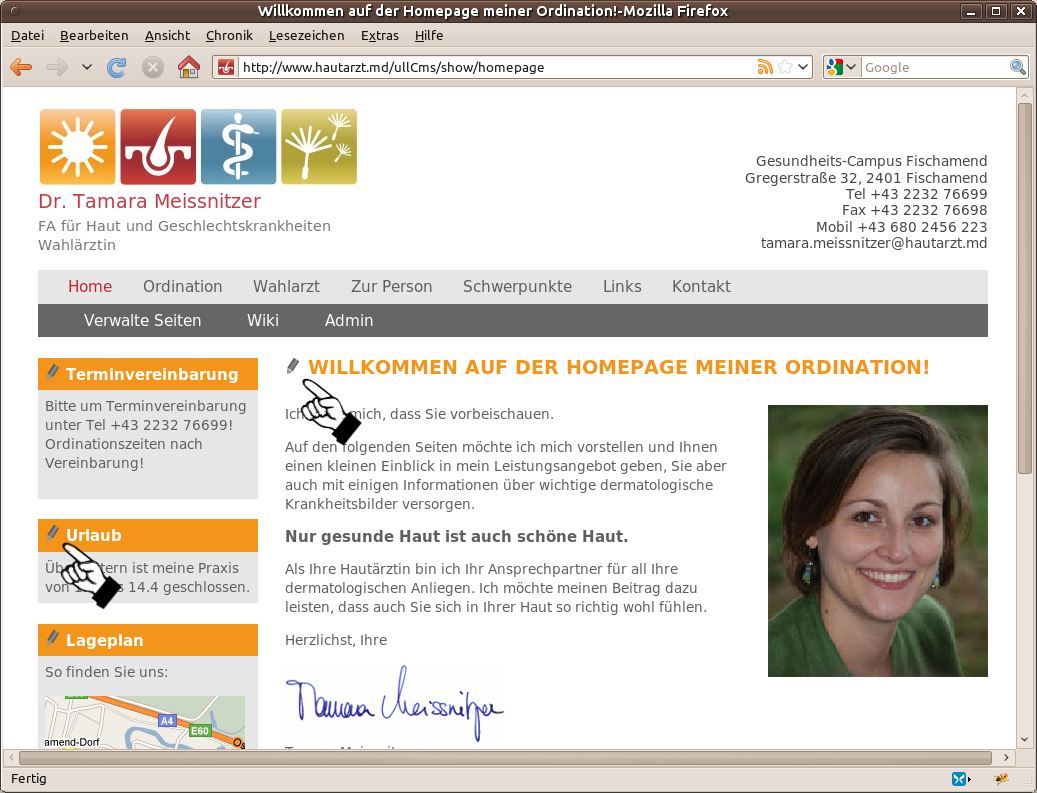
\includegraphics[width=0.9\textwidth]{direct_edit}
\caption{Icons zur direkten Bearbeitung}
\label{fig:direct_edit}
\end{figure}

Wenn Sie angemeldet sind und die nötigen Berechtigungen besitzen erscheint vor jeder Überschrift ein Stiftsymbol (Icon) (Siehe Abbildung \vref{fig:direct_edit}). Durch Klick auf das Icon können Sie den entsprechenden Text sofort bearbeiten.

Näheres zur Bearbeitung selbst erfahren Sie im Kapitel \vref{sec:edit}.




\section{Seiten verwalten}

Klicken Sie in der Admin-Menüleiste auf den Menüpunkt "`Seiten verwalten"'. Sie sehen nun eine Liste aller CMS-Seiten (Abbildung \vref{fig:list}):

\begin{figure}[htp]
\centering

\includegraphics[width=0.9\textwidth]{list}
\caption{Liste aller CMS-Seiten}
\label{fig:list}
\end{figure}


\subsection{Spalten}

Folgende Spalten werden in der Liste angezeigt:

\begin{itemize}
\item Titel der Seite
\item Übergeordneter Menüeintrag - Also wo die Seite in der Struktur der Webseite plaziert ist. Beispiele: "`Hauptmenü"', "`Fußzeile"' oder als Untermenüpunkt wie z.B. die Seite "`Anfängerkurse"' als Unterpunkt von "`Kurse"'.
\item Ist aktiv - Der Status der Seite. Inaktive Seiten werden den Besuchern nicht angezeigt.
\item Aktualisiert von - Wer die Seite zuletzt bearbeitet hat
\item Aktualisiert am - Wann die Seite zuletzt bearbeitet wurde
\end{itemize}


\subsection{Sortieren}

Klicken Sie auf eine Spaltenüberschrift wie zum Beispiel "`Aktualisiert am"' um die Liste nach diesem Feld zu sortieren. Klicken Sie nochmal auf die gleiche Spaltenüberschrift um die Sortierung umzukehren.


\subsection{Blättern}

Bei einer großen Anzahl an Seiten werden nicht alle Einträge auf einer Seite angezeigt. Benutzen Sie in diesem Fall die "`Blättern"' Funktion um weitere Seiten aufzurufen (Abbildung \vref{fig:paging}).

\begin{figure}[htp]
\centering
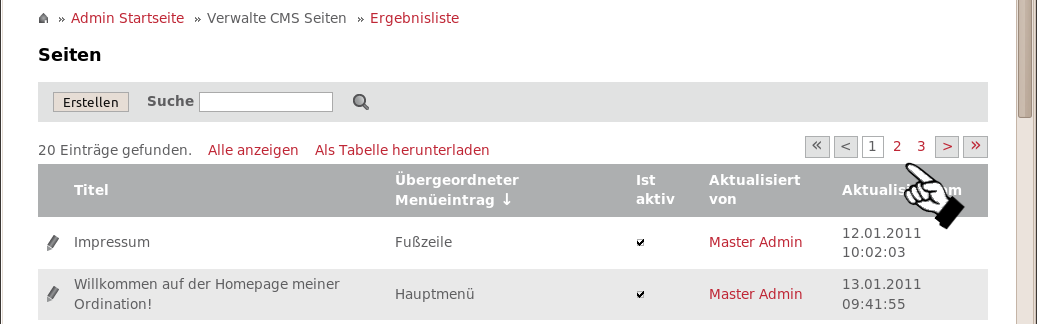
\includegraphics[width=0.9\textwidth]{paging}
\caption{Blättern}
\label{fig:paging}
\end{figure}


\subsection{Suche}

Wenn Ihre Webseite aus vielen Seiten besteht kann die Suchfunktion (Abbildung \vref{fig:search}) hilfreich sein .

Geben Sie eine Suchbegriff oder auch nur einen Teil davon in das Suchfeld ein und drücken sie [ENTER] oder klicken Sie das Lupen-Symbol an.
Die Liste beschränkt sich nun auf die Seiten, die den Suchbegriff im Betreff enthalten. Der Suchbegriff erscheint zusätzlich als "`Filter"'. Durch Klick auf das Papierkorb-Symbol entfernen Sie das Filterkriterium.

\begin{figure}[htp]
\centering
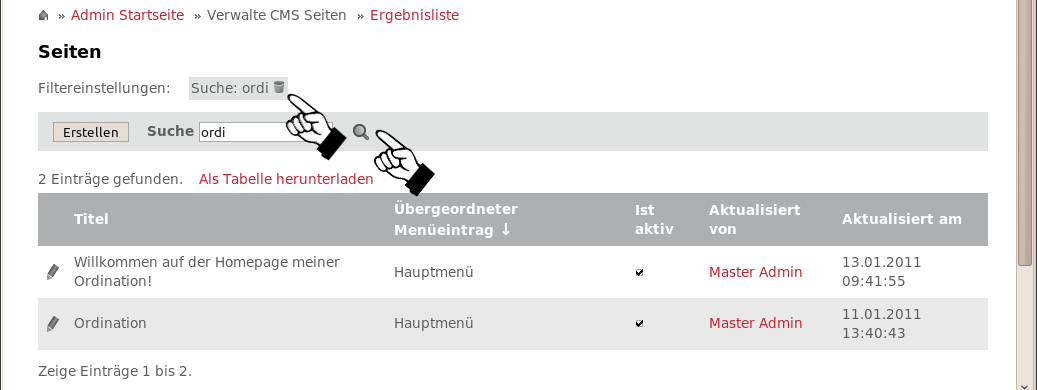
\includegraphics[width=0.9\textwidth]{search}
\caption{Suche}
\label{fig:search}
\end{figure}



\subsection{Neue Seite erstellen}

Klicken Sie auf "`Erstellen"' um eine neue CMS-Seite zu erstellen. Alles weitere erfahren Sie im Kapitel \vref{sec:edit}.


\section{Seiten bearbeiten}
\label{sec:edit}

\begin{figure}[htp]
\centering
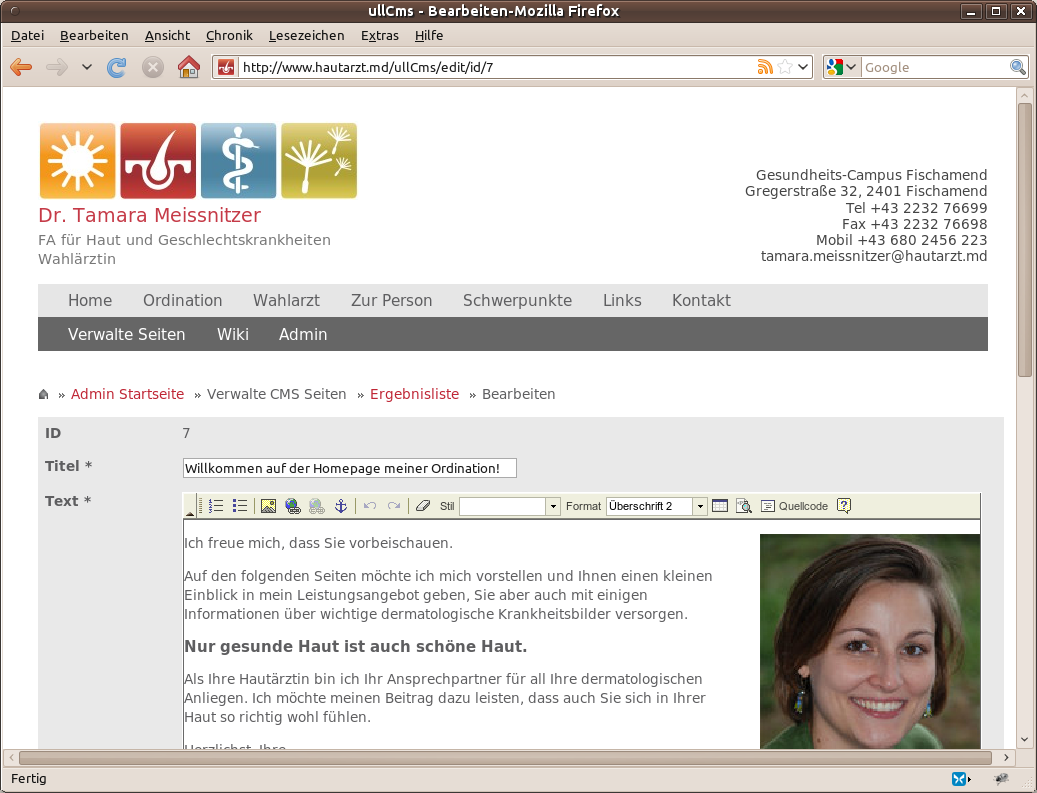
\includegraphics[width=0.9\textwidth]{edit1}
\caption{Bearbeiten Teil 1}
\label{fig:edit1}
\end{figure}

\begin{figure}[htp]
\centering
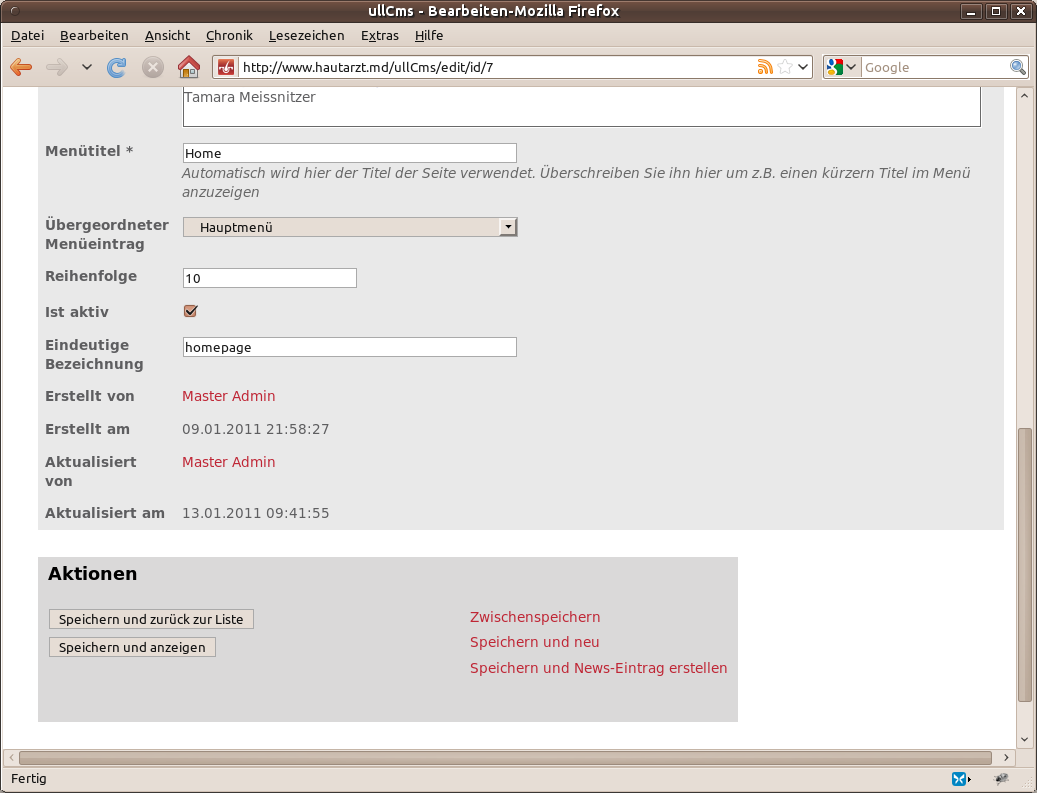
\includegraphics[width=0.9\textwidth]{edit2}
\caption{Bearbeiten Teil 2}
\label{fig:edit2}
\end{figure}

\subsection{Titel}

Der Titel Ihrer Seite wie er auf der Seite selbst als Überschrift angezeigt werden soll.

\subsection{Text}

ullCms bietet einen komfortablen
Editor, der ähnlich wie OpenOffice Writer oder MS Word funktioniert.
Auch das Einfügen von Bildern oder Anhängen ist einfach möglich. 

Alles rund um die Bedienung des Editors erfahren Sie im Kapitel \vref{sec:editor}.

\subsection{Menütitel}

Der Titel des Seite für die Anzeige in einem Menü. Standardmäßig wird hier der Titel übernommen. Es kann aber sinnvoll sein einen z.B. kürzeren Titel für die Menüs zu verwenden.

\subsection{Übergeordneter Menüeintrag}

Wählen Sie hier an welchem Punkt der Struktur Ihrer Webseite die aktuelle seite plaziert wird. Beispiele: "`Hauptmenü"', "`Fußzeile"' oder als Untermenüpunkt wie z.B. die Seite "`Anfängerkurse"' als Unterpunkt von "`Kurse"'.

\subsection{Reihenfolge}

Normalerweise werden die einzelnen Einträge in einem Menü wie z.B. dem Hauptmenü alphabetisch sortiert. In dieses Feld können sie ganze Zahlen eingeben um die Sortierung zu beeinflussen. Tipp: verwenden sie ganze 10er oder 100er Zahlen um später Einträge einfügen zu können. 

\subsection{Ist aktiv}

Der Status der Seite. Setzen Sie den Status auf "`Inaktiv"' um eine Seite den Besuchern nicht mehr anzuzeigen.

\subsection{Eindeutige Bezeichnung}

Der Name der Seite wie er in der Adresszeile (URL) angezeigt wird. Beispiel: "'anfaenger-kurse"`.

\subsection{Aktionen}

Für das Bearbeiten oder Erstellen mehrerer Seiten bietet ullCms einige praktische Aktionen:

\begin{itemize}
\item Speichern und zurück zur Liste - Sie gelangen wieder zur Liste der Seiten
\item Speichern und anzeigen - Die eben bearbeitete Seite aus der Sicht der Besucher ansehen
\item Zwischenspeichern - Auf der Bearbeitunsseite bleiben
\item Speichern und neu - Unmittelbar mit der Eingabe der Inhalte einer neuen Seite beginnen
\item Speichern und News-Eintrag erstellen - Wenn Sie das ullNews Modul verwenden können Sie hier direkt einen neuen News-Eintrag erstellen der zur eben bearbeiteten CMS-Seite verlinkt ist
\end{itemize}

\section{Text bearbeiten mit dem "`WYSIWYG"' Editor}
\label{sec:editor}

"`WYSIWYG"' steht für "`What you see is what you get"' also dass man schon bei der Eingabe sieht wie der Text letztendlich aussehen wird.

\begin{figure}[htp]
\centering
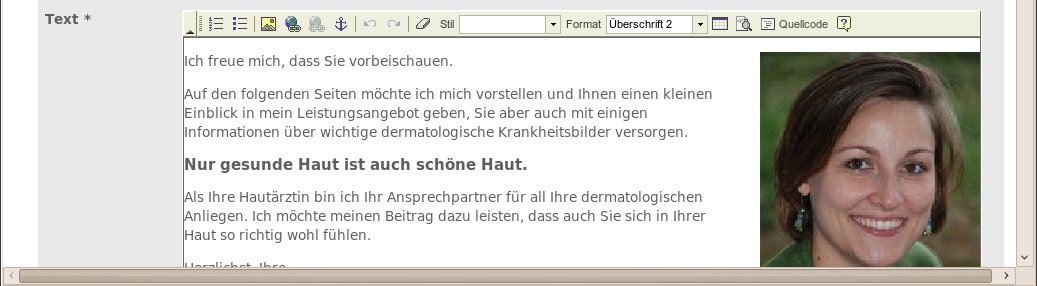
\includegraphics[width=0.9\textwidth]{editor}
\caption{WYSIWYG-Editor}
\label{fig:editor}
\end{figure}

\subsection{Text schreiben}

Geben Sie wie von anderen Texteditoren gewohnt den Text ein.

Tipp: [Enter] erzeugt einen neuen Paragrafen, also einen Textblock mit einer Leerzeile dahinter. Einen einfachen Zeilenumbruch erreichen Sie mit [SHIFT - Enter].

\subsection{Text formatieren}

Markieren Sie den gewünschten Text und wählen Sie aus der Editor-Menüleiste die gewünschte Auszeichnung.

Bitte beachten Sie, dass die von uns ausgewählten
Formatierungsmöglichkeiten nach semantischen Gesichtspunkten ausgewählt
wurden. Sie finden also nur „logische“ Auszeichnungen wie zum Beispiel
„wichtig“ oder „Überschrift“, und keine rein optischen
Formatierungsmöglichkeiten wie Farben oder Schriftgrößen. Somit werden
saubere und zukunftssichere Texte gewährleistet. (Stichwort "`semantic
Web"')

Die wichtigsten Formatierungen (von links nach rechts):

\begin{itemize}
\item Nummerierte Liste
\item Liste mit Aufzählungszeichen
\item Stile: "`Important"' - also "`Wichtig"' wird fett angezeigt
\item Format: "`Überschrift"'
\end{itemize}


\subsection{Bild einfügen}

\begin{itemize}
\item Setzten Sie den Cursor an die gewünschte Stelle im Text
\item Klicken Sie auf das Bildsymbol 
\includegraphics[height=5mm]{image_icon}
\item Wählen Sie "`Server durchsuchen"'
\item Wählen oder erstellen Sie gegebenenfalls einen neuen Ordner um eine ordentliche Struktur Ihrer Daten zu gewährleisten
\item Wenn Sie ein neues Bild hochladen möchten klicken Sie auf "`Durchsuchen"' und wählen Sie eine Bilddatei von Ihrem Computer aus.
\item Vergessen Sie nicht danach auf "`Upload"' zu klicken
\item Wählen Sie nun ein Bild aus der Liste durch anklicken.
\item Klicken Sie auf "`OK"'
\end{itemize}

\subsection{Bildeigenschaften ändern}

Klicken Sie mit der rechten Maustaste auf das Bild und wählen Sie "`Bildeigenschaften"'.

Im folgenden werden die wichtigsten Eigenschaften erklärt:

\subsubsection{Reiter "`Bild-Info"'}

\begin{itemize}
\item Breite / Höhe - Wählen Sie die gewünschte Größe des Bildes in Pixel. Bitte beachten Sie, dass Bilder bereits vor dem Hochladen mit einem Grafikprogramm auf die endgültige Größe skaliert werden sollten
\item Ausrichtung - Wählen Sie "`Links"' oder "`Rechts"' wenn der Text das Bild umfließen soll.
\end{itemize}

\subsubsection{Reiter "`Erweitert"'}

Wenn Sie das Bild vom Text umfließen lassen ist häufig auf gewissen Seiten des Bildes ein Abstand erwünscht.
Dieser Abstand kann im Feld "`Style"' angegeben werden. Beispiel für einen Abstand links und unten: "`margin-left: 1.5em; margin-bottom: 1.5em;"'


\subsection{Link erstellen}

Normale Webadressen und E-Mailadressen werden in der normalen Ansicht für die Besucher der Webseite automatisch verlinkt.

Beispiele:

\begin{itemize}
\item www.ullright.org
\item http://ull.at
\item office@ull.at
\end{itemize}

Möchten Sie hingegen gewisse Wörter im Text verlinken markieren Sie die Wörter und klicken Sie auf das Linksymbol 
\includegraphics[height=5mm]{link_icon} (blau-grüne Erdkugel).

\subsubsection{Link zu einer Internetadresse (URL)}
Geben Sie bei "`URL"' die gewünschte Adresse ein. Beispiel: http://www.ullright.org

Bei Links zu Internetseiten empfiehlt sich die Seite in einem neuen Browserfenster zu öffnen. Wählen Sie hierzu im Reiter "`Zielseite"' "`Neues Fenster (\_blank)"'.

Zusätzlich empfehlen wir einen solchen Link durch das Symbol für "`Externe Seite"' zu kennzeichen. Schreiben Sie dazu im Reiter "`Erweitert"' die Anweisung "`link\_external"' in das Feld "`Stylesheet Klasse"'.

\subsubsection{Link zu einer anderen CMS-Seite}

Öffnen Sie die Zielseite in einem neuen Browsertab oder -fenster und kopieren Sie die Adresse.

Beispiel: http://www.ull.at/ullCms/show/kontakt

Geben Sie nun bei "`URL"' die gekürzte Adresse startend mit den Schrägstrich nach dem Domänennamen ein.

Beispiel: /ullCms/show/kontakt

\subsubsection{E-Mail Link}

Wählen Sie bei "`Link-Typ"' E-Mail und geben Sie die gewünschte E-Mailadresse ein.



\subsection{Datei hochladen}

Das Hochladen einer Datei funktioniert wie eine Mischung aus Link- und Bildeinfügen.

\begin{itemize}
\item Markieren Sie die Wörter die mit der Datei verlinkt werden sollen.
\item Klicken Sie auf das Linksymbol 
\includegraphics[height=5mm]{link_icon} (blau-grüne Erdkugel)
\item Wählen Sie „Server durchsuchen“
\item Wählen oder erstellen Sie gegebenenfalls einen neuen Ordner um eine ordentliche Struktur Ihrer Daten zu gewährleisten
\item Wenn Sie eine neue Datei hochladen möchten klicken Sie auf "`Durchsuchen"' und wählen Sie eine Datei von Ihrem Computer aus.
\item Vergessen Sie nicht danach auf "`Upload"' zu klicken
\item Wählen Sie nun die Datei aus der Liste durch anklicken.
\item Klicken Sie auf „OK“
\end{itemize}








\end{document}